\documentclass[14pt]{beamer}
\usetheme{default}
\usecolortheme{dove}

\title[EPDM Presentation]{Part 4-1 \\ Response Surface Methodology}
\author[C. L. Quale]{Christian Leonard Quale}
\institute{
  University of Edinburgh
}
\date[January 2013]{January, 2013}


\begin{document}

\begin{frame}[plain]
  \titlepage
\end{frame}



\begin{frame}{Response Surface Methodology - Why?}

Necessity: \\
\pause
\ \\
\ \\
\begin{columns}
    \begin{column}{0.5\textwidth}
      \centering
      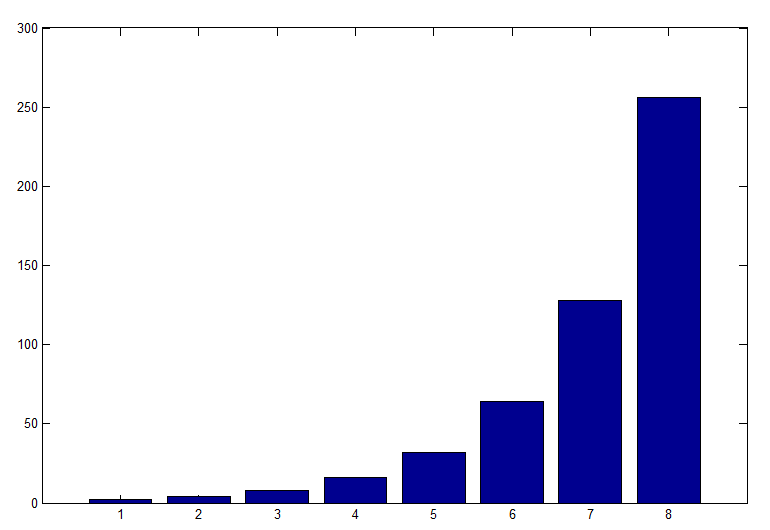
\includegraphics[width=1.1\textwidth]{2levels.png}
    \end{column}
    \pause
    \begin{column}{0.5\textwidth}
      \centering
      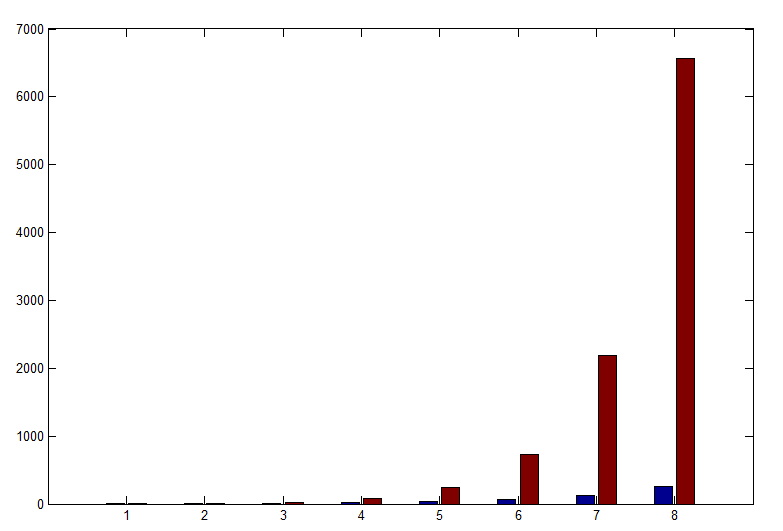
\includegraphics[width=1.1\textwidth]{3levels.png}
    \end{column}
  \end{columns}

\end{frame}

\begin{frame}{Response Surface Methodology}
\pause
\begin{itemize}
\item Create specialised experimental models
\pause
\item Perform a regression on results
\pause
\item Create a simplified mathematical model:
\end{itemize}
\pause
\begin{center}
{\small $Y = a_0+a_1X1 + a_2X2 + a_3X1X2 + a_4X1^2+a_5X2^2 + Error$}
\end{center}
\end{frame}

\begin{frame}{Response Surface Methodology}
Theoretical Model:
{\small $$ Y=\frac{15.0X1^2}{1.0+1.5e^{2.5X2}} $$}
\pause
Quadratic Approximation: \\
\ \\
{\small $Y = a_0+a_1X1 + a_2X2 + a_3X1X2 + a_4X1^2+a_5X2^2$ \\
\ \\
\pause
$a_0 = 14.92$ \hspace{1cm} $a_1 = 7.65$ \hspace{1cm} $a_2 = -16.76$ \hspace{1cm} $a_3 = 0.77$ \hspace{1.197cm} $a_4 = -6.53$ \hspace{0.665cm} $a_5 = 6.31$\\
\ \\
\begin{center}$2 \leq X1 \leq 3$ \hspace{2cm} $0\leq X2\leq1$\end{center}}
\end{frame}


\begin{frame}{Response Surface Methodology}

Quadratic Approximation: \\
{\small $Y = 14.92+7.65X1  -16.76X2 + 0.77X1X2  -6.53X1^2+6.31X2^2$ \\

\ \\
\begin{center}$2 \leq X1 \leq 3$ \hspace{2cm} $0\leq X2\leq1$\end{center}}
\pause
\begin{columns}
    \begin{column}{0.5\textwidth}
    Theoretical Model:

      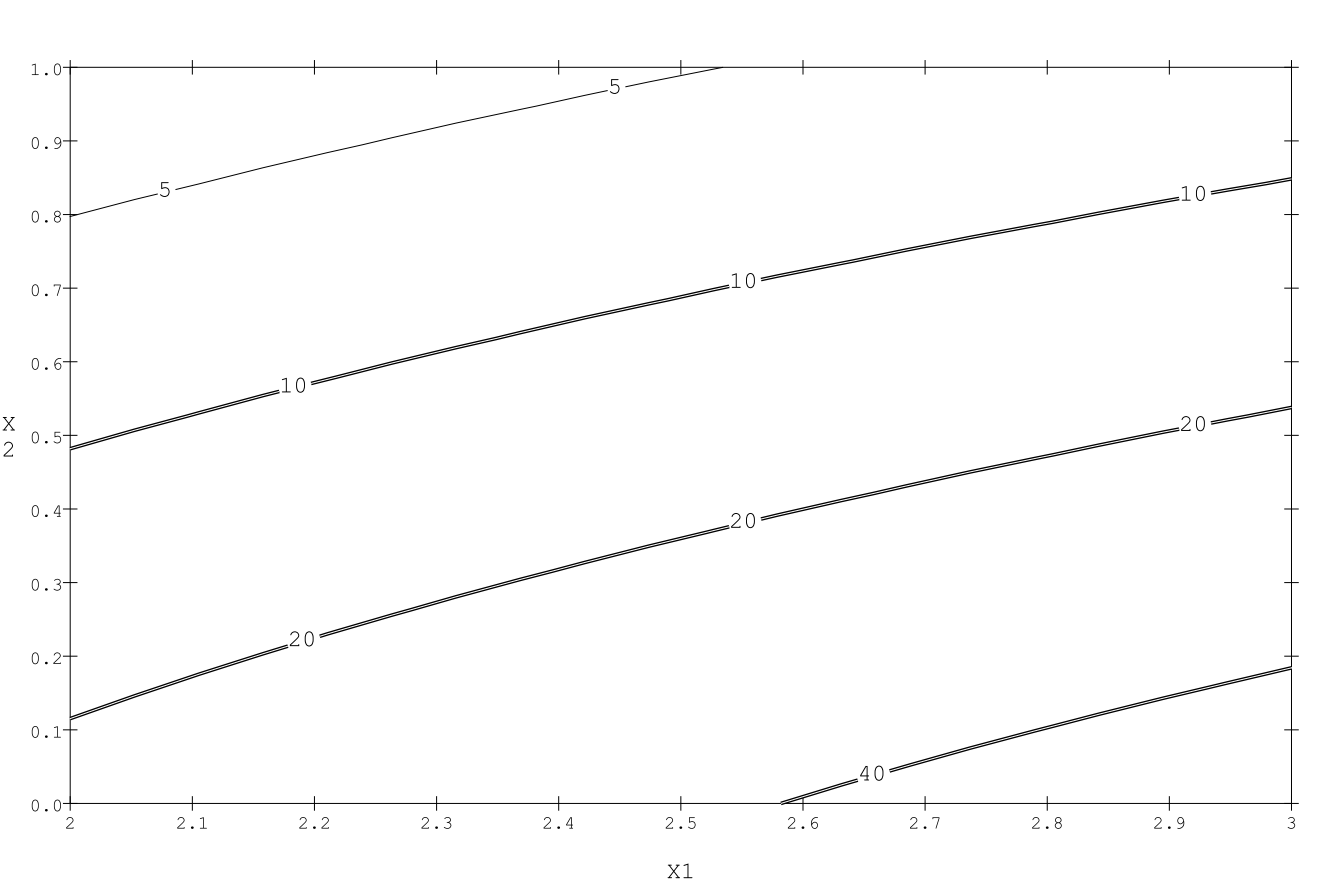
\includegraphics[width=1.1\textwidth]{actualgraph.png}
    \end{column}
    \pause
    \begin{column}{0.5\textwidth}
      Approximation:

      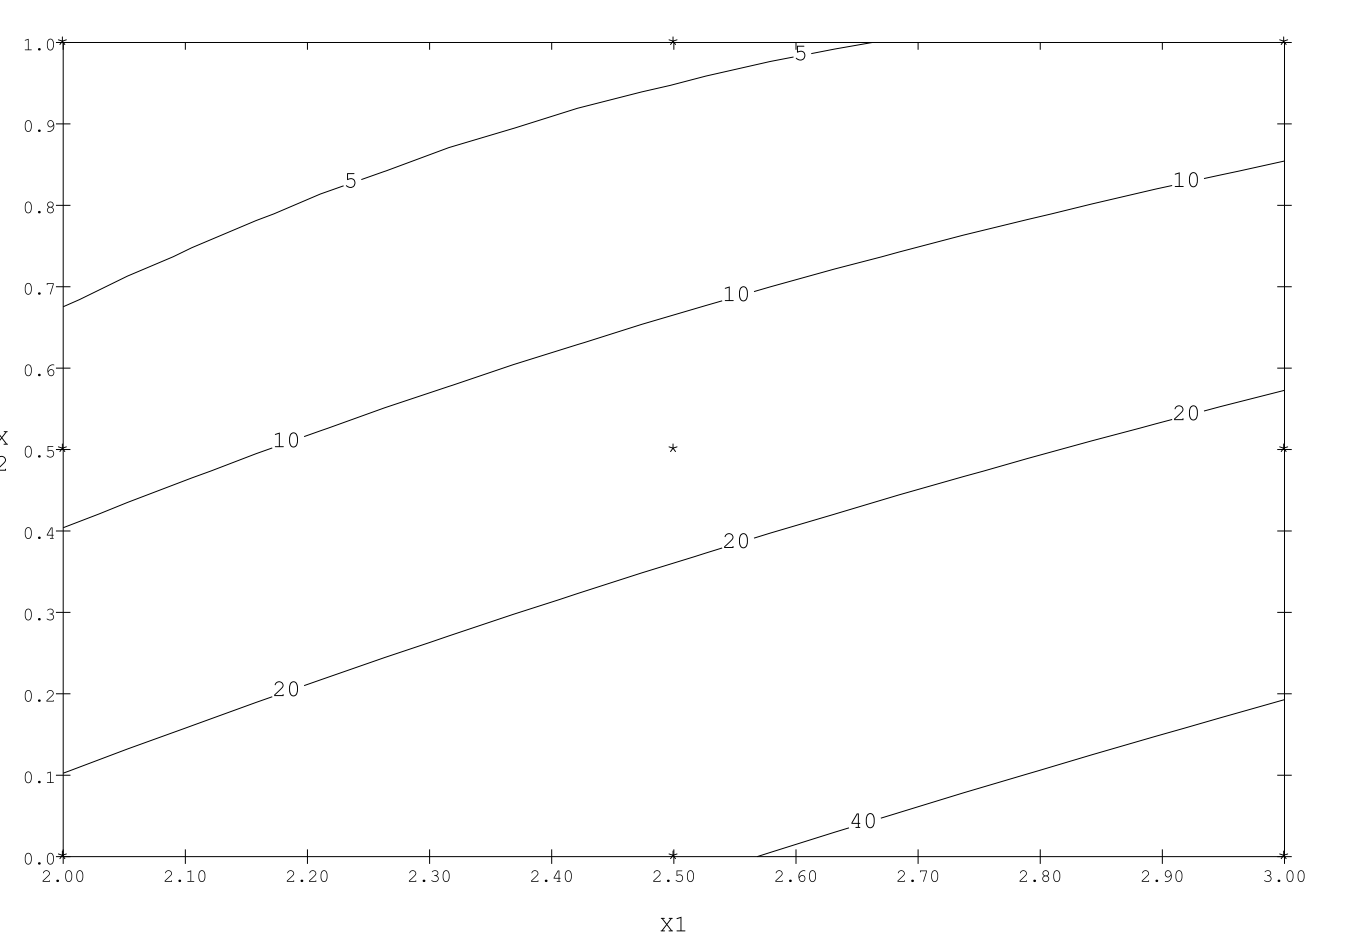
\includegraphics[width=1.1\textwidth]{modelgraph.png}
    \end{column}
  \end{columns}

\end{frame}

\begin{frame}{Response Surface Methodology}

\begin{columns}
    \begin{column}{0.5\textwidth}
    Theoretical Model:

      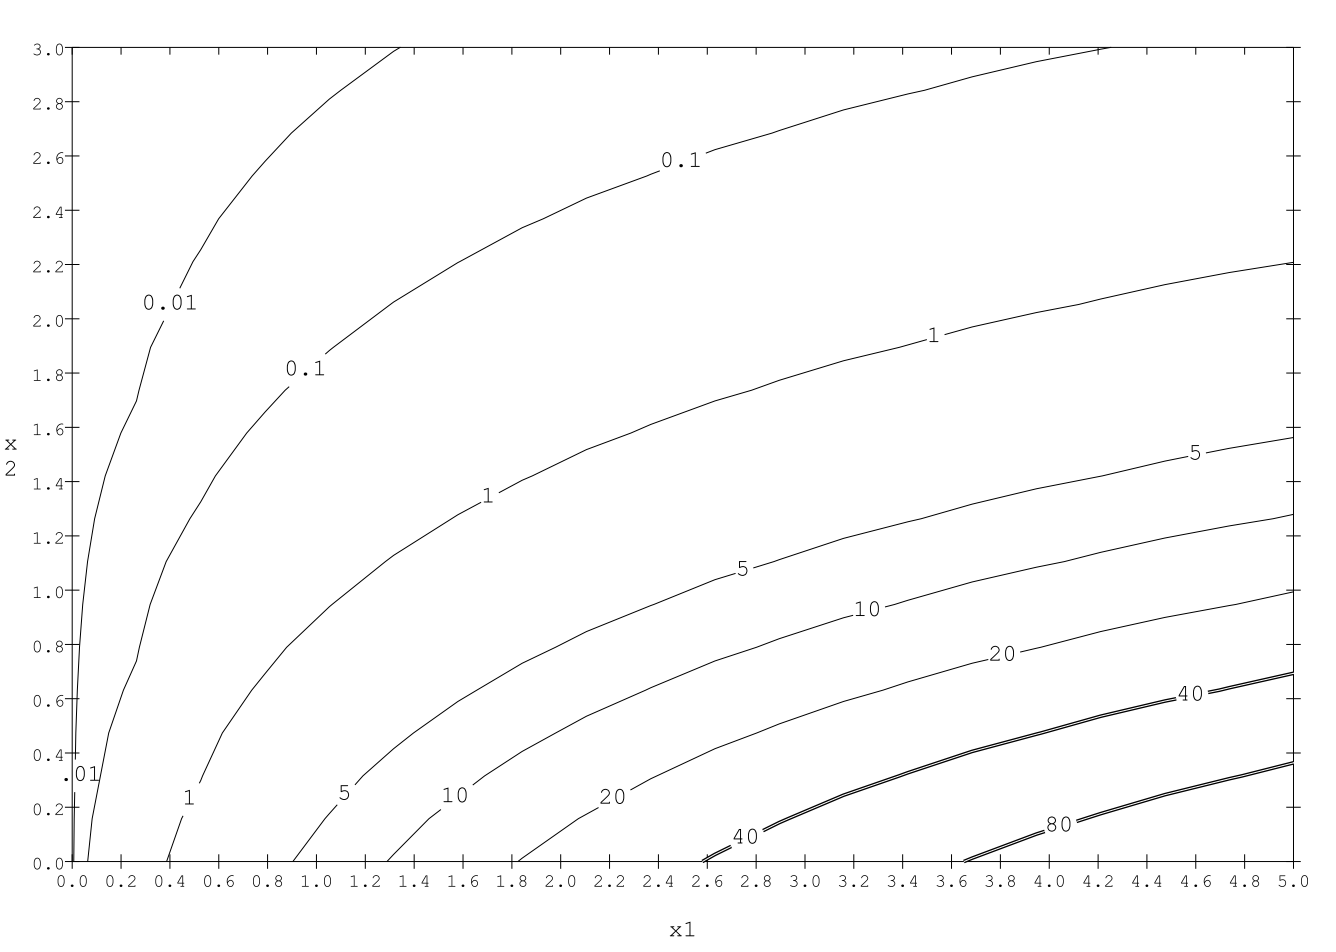
\includegraphics[width=1.1\textwidth]{actualgraphout.png}
    \end{column}
    \begin{column}{0.5\textwidth}
      Approximation:

      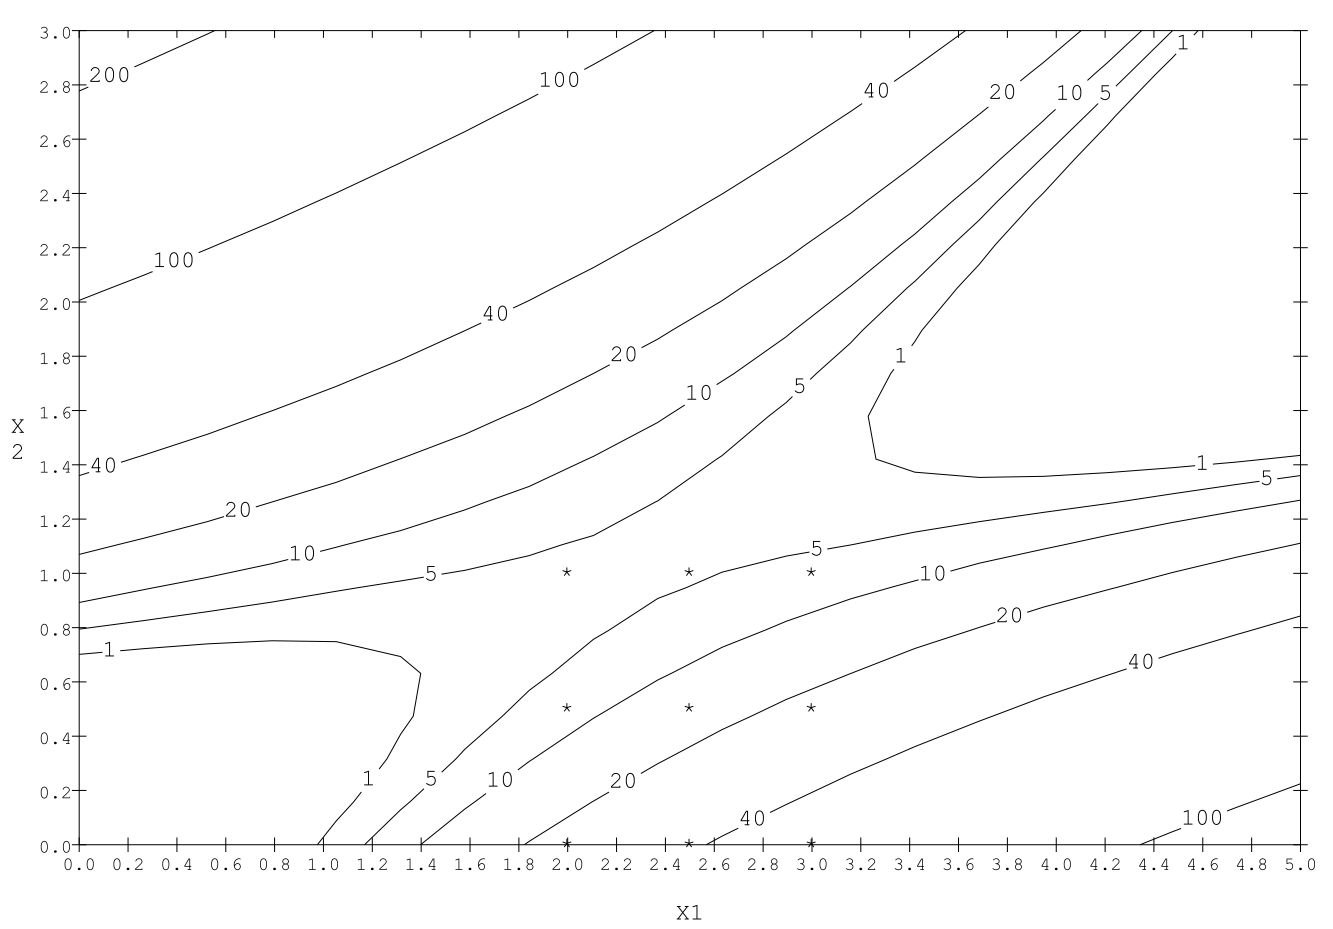
\includegraphics[width=1.1\textwidth]{modelgraphout.png}
    \end{column}
  \end{columns}

\end{frame}

\begin{frame}{Central Composite Designs}
\pause
\begin{itemize}
\item Based on Fractional Factorial Designs
\vspace{0.5cm}
\pause
\item Creates a new design suitable for regression
\vspace{0.5cm}
\pause
\item Software kindly designs experimental models for us
\end{itemize}
\vspace{1cm}
\pause
Good basis for regressions: Rotatable Designs


\end{frame}

\begin{frame}{Rotatable Designs}
\pause
\begin{center}
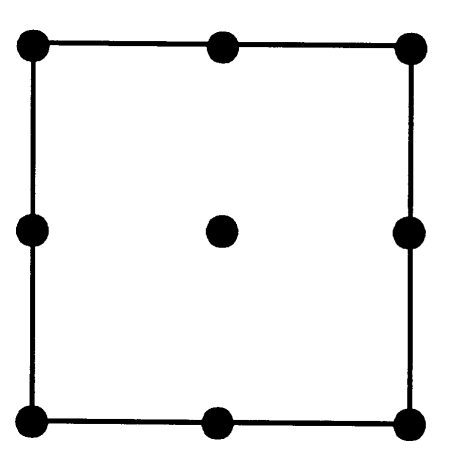
\includegraphics[width=0.5\textwidth]{3level2factor.png}
\end{center}
\end{frame}

\begin{frame}{Rotatable Designs}
\begin{center}
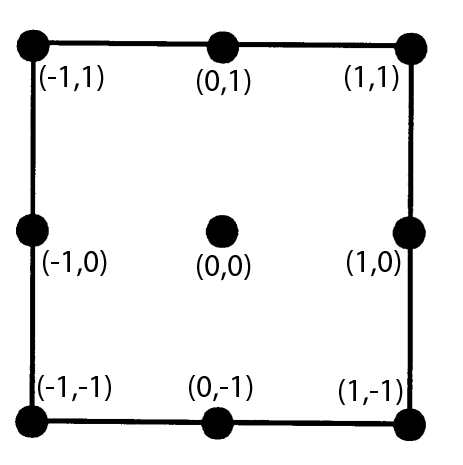
\includegraphics[width=0.5\textwidth]{3level2factoranno.png}
\end{center}
\end{frame}

\begin{frame}{Rotatable Designs}
\begin{center}
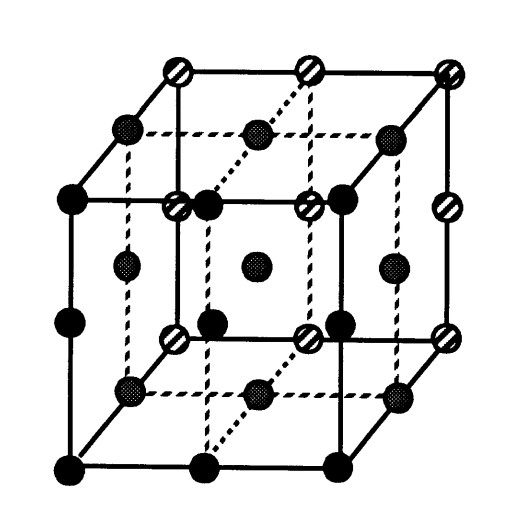
\includegraphics[width=0.5\textwidth]{3level3factor.png}
\end{center}
\end{frame}

\begin{frame}{Rotatable Designs}
\begin{center}
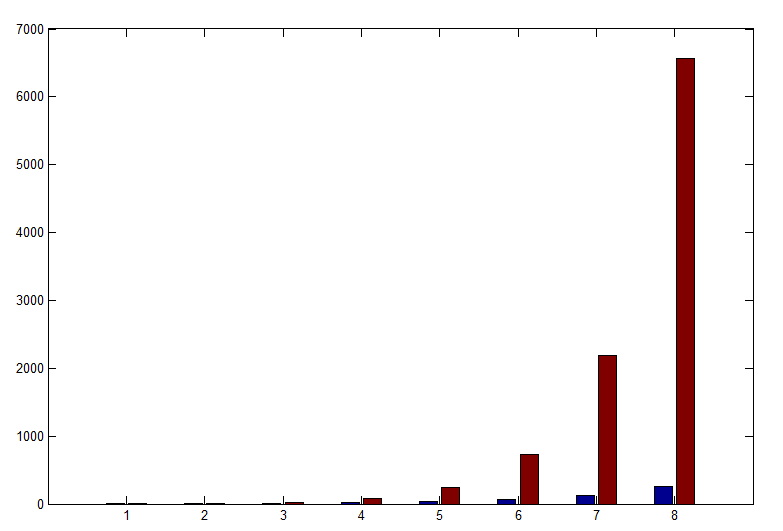
\includegraphics[width=0.9\textwidth]{3levels.png}
\end{center}
\end{frame}

\begin{frame}{Rotatable Designs}
\pause
\begin{columns}
    \begin{column}{0.5\textwidth}
      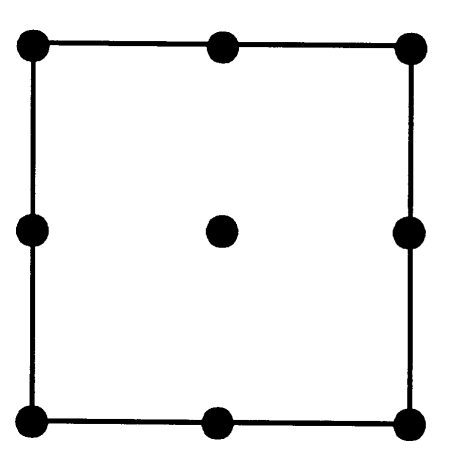
\includegraphics[width=0.9\textwidth]{3level2factor.png}
      \pause
    \end{column}
    \begin{column}{0.5\textwidth}
      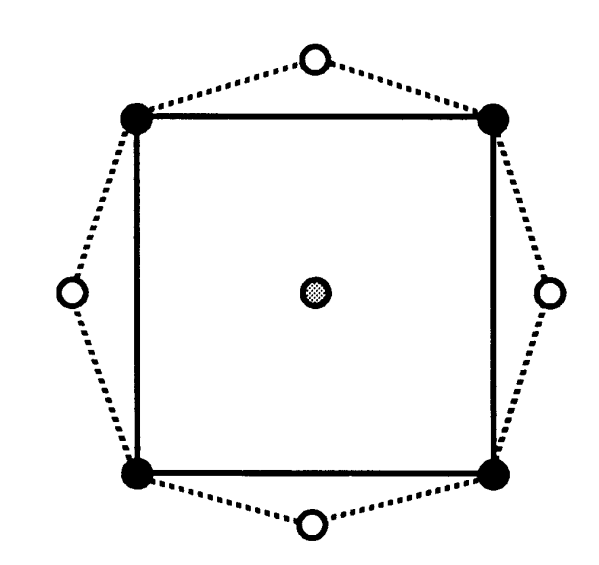
\includegraphics[width=1.1\textwidth]{3level2factorCCI.png}
    \end{column}
  \end{columns}
\end{frame}

\begin{frame}{Rotatable Designs}
\begin{columns}
    \begin{column}{0.5\textwidth}
      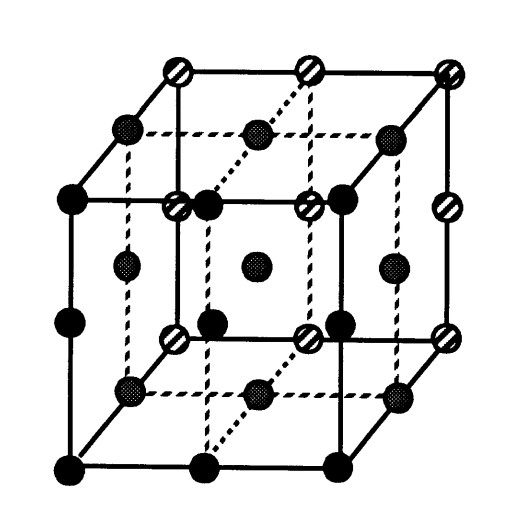
\includegraphics[width=1.1\textwidth]{3level3factor.png}
    \end{column}
    \begin{column}{0.5\textwidth}
      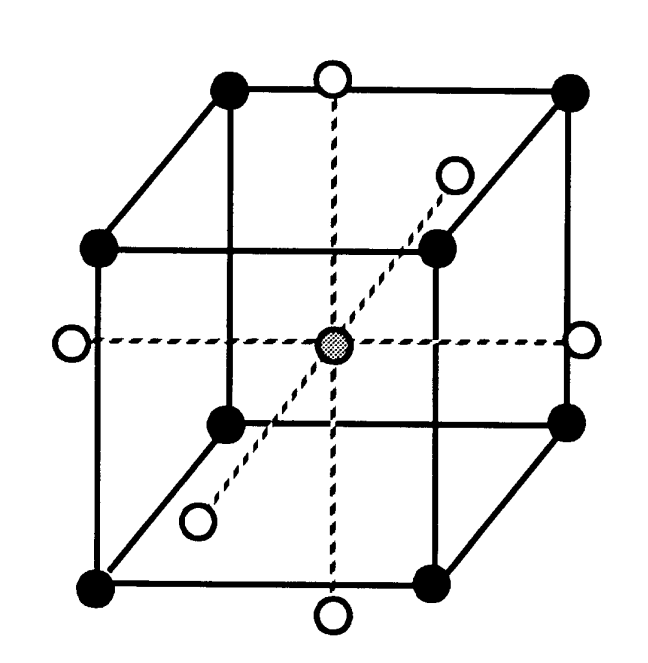
\includegraphics[width=1.1\textwidth]{3level3factorCCI.png}
    \end{column}
  \end{columns}
\end{frame}

\begin{frame}{Rotatable Designs}
\begin{columns}
    \begin{column}{0.5\textwidth}
      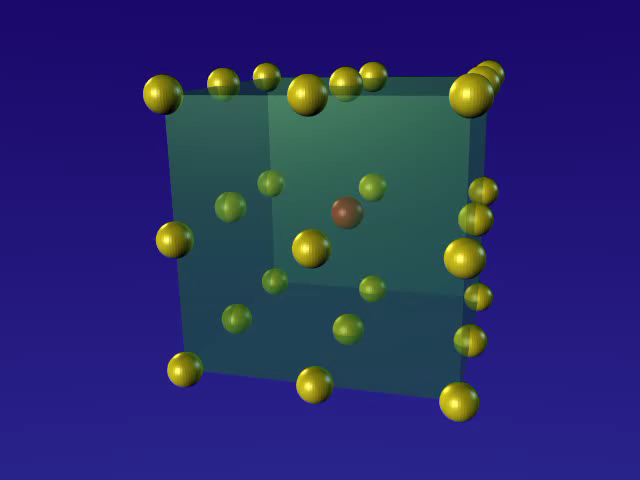
\includegraphics[width=1.1\textwidth]{3level3factor3D.png}
    \end{column}
    \begin{column}{0.5\textwidth}
      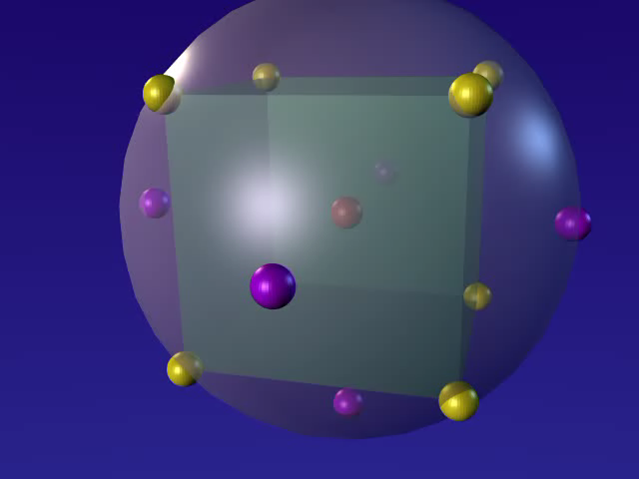
\includegraphics[width=1.1\textwidth]{3level3factorCCI3D.png}
    \end{column}
  \end{columns}
\end{frame}

\begin{frame}{Central Composite Circumscribed Design}

\begin{columns}
    \begin{column}{0.5\textwidth}
      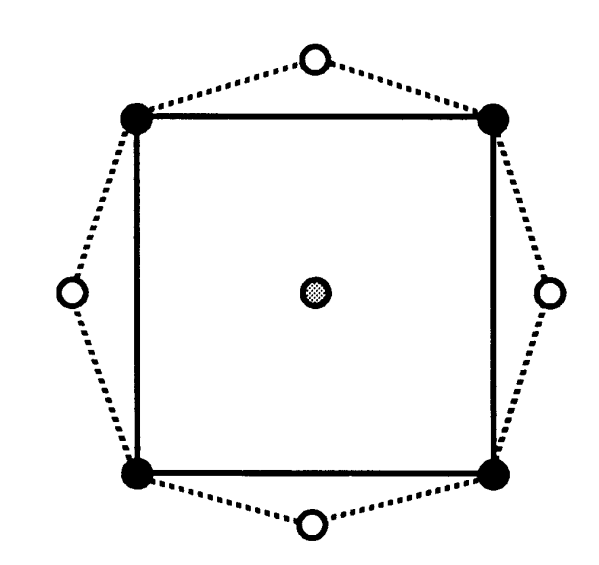
\includegraphics[width=0.9\textwidth]{3level2factorCCI.png}
    \end{column}
    \begin{column}{0.5\textwidth}
      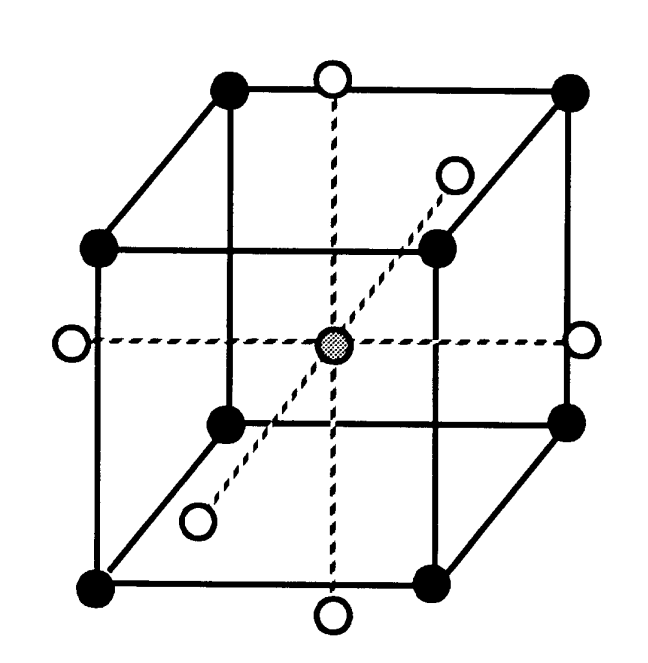
\includegraphics[width=1.1\textwidth]{3level3factorCCI.png}
    \end{column}
  \end{columns}

\end{frame}

\begin{frame}{Central Composite Circumscribed Design}
\pause
\begin{itemize}
\item Need access to 5 levels
\pause
\item Need access above and below previously defined Max/Min points
\end{itemize}

\end{frame}

\begin{frame}{Central Composite Circumscribed Design}

\begin{columns}
    \begin{column}{0.5\textwidth}
      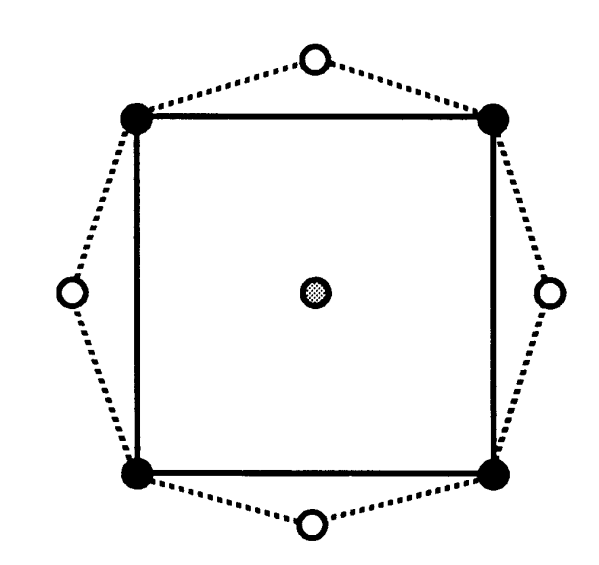
\includegraphics[width=0.9\textwidth]{3level2factorCCI.png}
    \end{column}
    \pause
    \begin{column}{0.5\textwidth}
      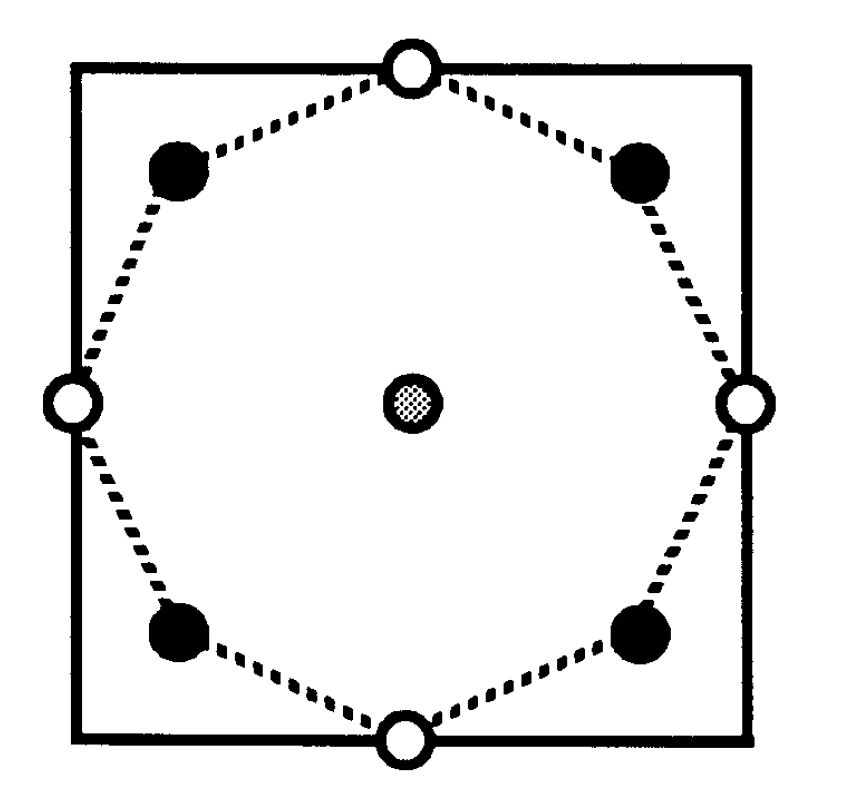
\includegraphics[width=0.7\textwidth]{3level2factorCCI2.png}
    \end{column}
  \end{columns}

\end{frame}

\begin{frame}{Central Composite Inscribed Design}

\begin{columns}
    \begin{column}{0.5\textwidth}
      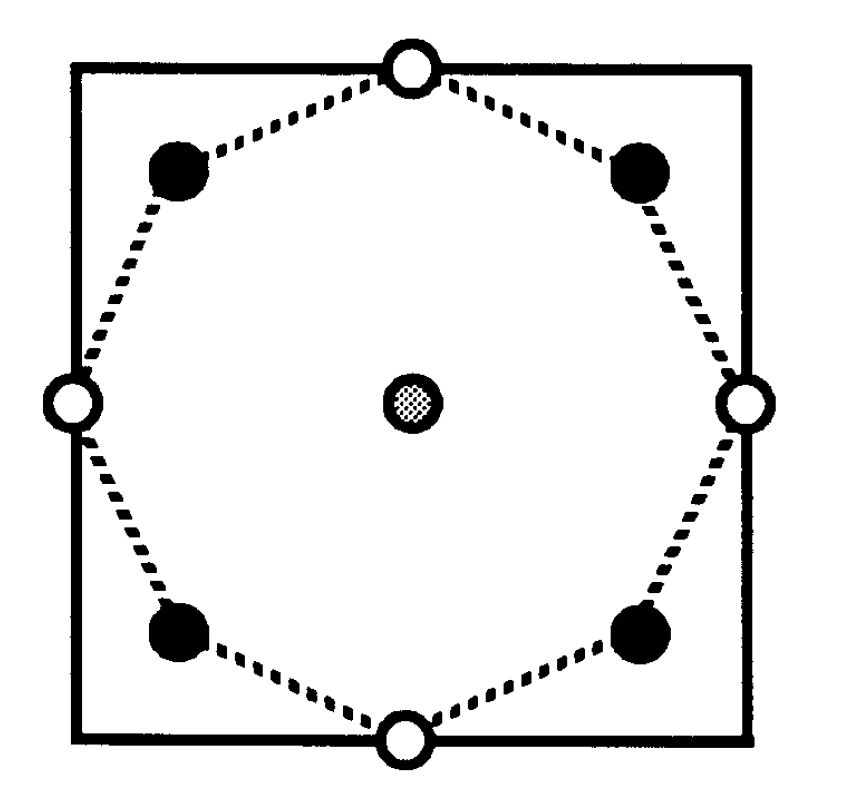
\includegraphics[width=0.9\textwidth]{3level2factorCCI2.png}
    \end{column}
    \pause
    \begin{column}{0.5\textwidth}
      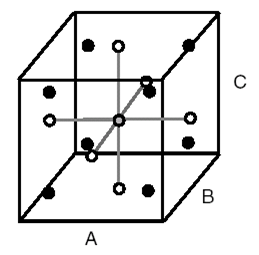
\includegraphics[width=0.9\textwidth]{3level3factorCCI2.png}
    \end{column}
  \end{columns}
\end{frame}

\begin{frame}{Central Composite Inscribed Design}
\begin{center}
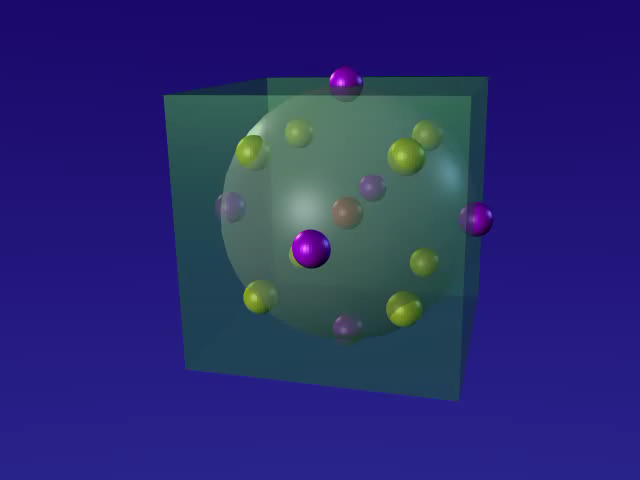
\includegraphics[width=0.7\textwidth]{3level3factorCCI23D.png}
\end{center}
\end{frame}


\begin{frame}{Central Composite Inscribed Design}
\pause
\begin{itemize}
\item Still need access to 5 levels
\pause
\item Fails to test extremities
\end{itemize}

\end{frame}

\begin{frame}{Face Centred Cube}
\pause

\begin{columns}
    \begin{column}{0.5\textwidth}
      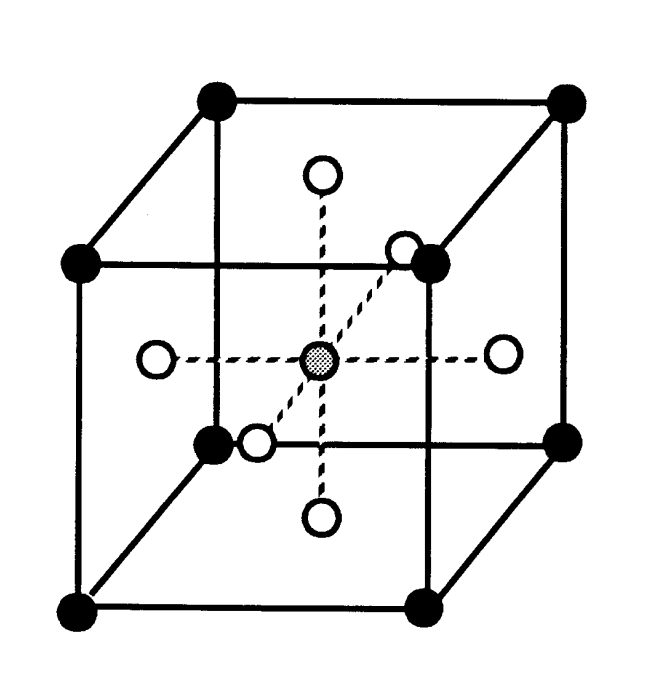
\includegraphics[width=0.9\textwidth]{CCF.png}
    \end{column}
    \pause
    \begin{column}{0.5\textwidth}
      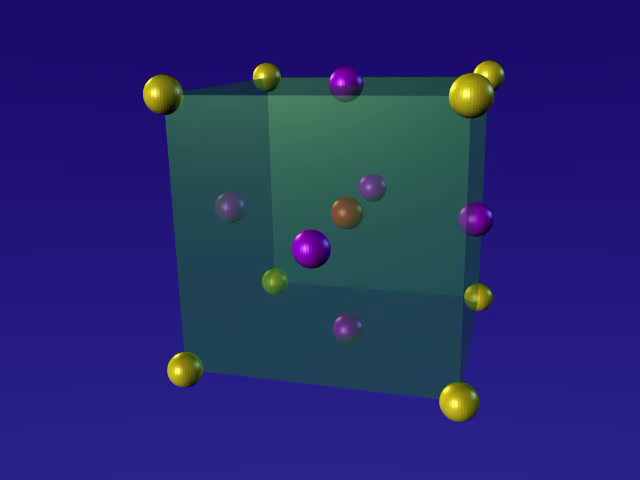
\includegraphics[width=0.9\textwidth]{CCF3D.png}
    \end{column}
  \end{columns}

\end{frame}

\begin{frame}{Face Centred Cube}
Kind of like CCC/CCI Designs...\\
\ \\
\pause
Only requires three levels.\\
\ \\
\pause
One Major disadvantage: \\
\pause
Not orthogonal! \\
\ \\
\vspace{3cm}
\pause
Wait, what? Orthogonal?
\end{frame}


\begin{frame}{Orthogonal Designs}
\pause
\begin{itemize}
\item Blockable
\pause
\item Can be run in batches
\pause
\item Divide experiments into groups
\end{itemize}
\pause
\ \\
\ \\
...even more options?
\end{frame}

\begin{frame}{Box Behnken Design}
\pause
\begin{columns}
    \begin{column}{0.5\textwidth}
      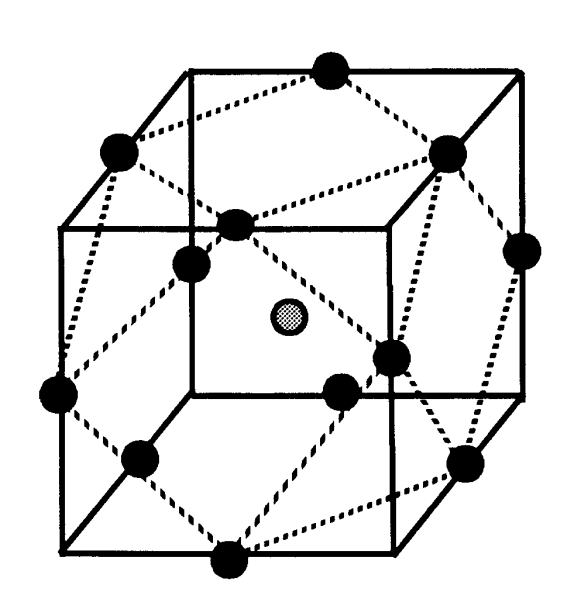
\includegraphics[width=0.9\textwidth]{BBD.png}
    \end{column}
    \pause
    \begin{column}{0.5\textwidth}
      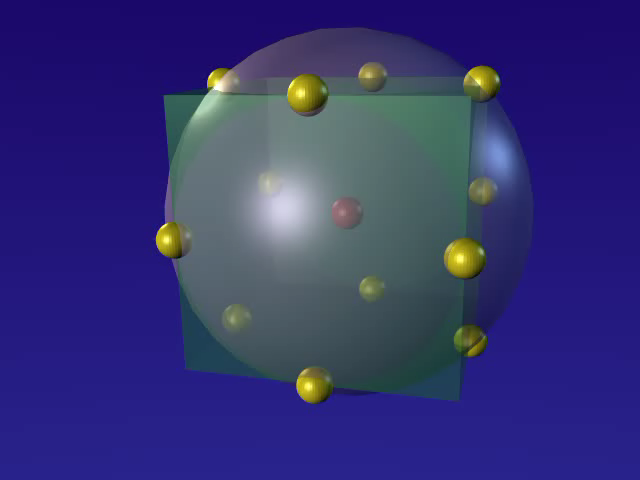
\includegraphics[width=\textwidth]{BBD3D.png}
    \end{column}
  \end{columns}
\end{frame}

\begin{frame}{D-Optimal Designs}
\pause
The computer sorts out everything!\\
\ \\
\ \\
\pause
Tell it how many runs you can afford, what regions you are interested in, and what model you prefer, and it will automatically design and optimal set of experimental runs for you. 
\end{frame}

\begin{frame}{Choices... Choices...}
\pause
How to choose?
\pause
\begin{itemize}
\item How close is the corner of the optimum operating region to the corner of the design region?
\pause
\item Do I care about orthogonality or rotatability?
\pause
\item Is it possible to experiment outside of the design-factor range?
\pause
\item How many runs can I afford?
\pause
\item What is my personal preference?
\end{itemize}
\end{frame}

\begin{frame}{Summary}
\pause

\begin{itemize}
{\normalsize
\item The ultimate goal is to create an RSM model.
\pause
\item  In the process of doing this we choose an experimental design to create a good RSM model.
\pause
\item Different designs are all different, but valid, ways of gathering data for this model.
\pause
\item Once a good model exists, no more experiments are necessary. The magic of statistics lets you predict the likely outcome of any combination of factors without running an experiment.

}
\end{itemize}

\end{frame}

\end{document}